\chapter{开放通道SSD与高性能应用}
\label{cha:ssd_hpc}

\section{开放通道SSD设备简介}
\subsection{SSD内部结构}
SSD,全称为固态硬盘(solid-state drive),是一种由多个闪存芯片组成的存储设备。本文主要关注由NAND闪存芯片组成的SSD,因为目前主流的SSD设备均采用NAND芯片,对NAND的管理与现实应用关系更加密切。

典型SSD设备的内部结构如图\ref{fig:ssd_geo}所示。SSD的控制器上并行连接了多组闪存芯片,每组闪存芯片一般包含数十个NAND存储芯片,并通过名为Channel的结构连接到控制器。每个Channel下的芯片按照Die、Plane、Block和Page的层级组织。一个Die每次只允许执行一个IO请求,即SSD并行执行IO请求的最小单元是Die。在开放通道SSD设备中,一个或者多个Die也会被合并称为一个Lun。每个Die含有相同数量的Plane,同样,每个Plane含有相同数量的Block,每个Block也含有相同数量的Page。每个Page还继续被分为固定大小的Sector,同时包含一个OOB区域(out-of-bound area)用于存储元数据。

\begin{figure}[H]
  \centering
  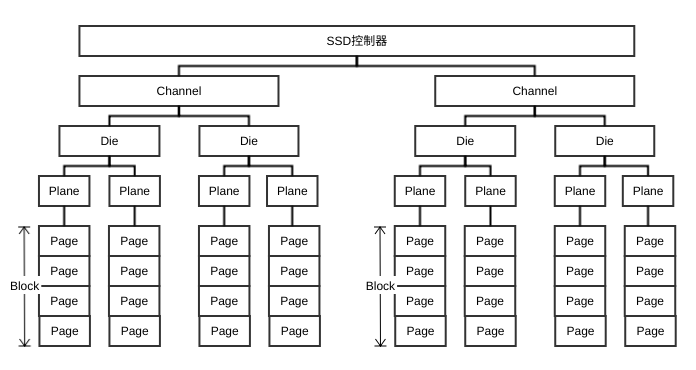
\includegraphics[width=0.8\textwidth]{ssdgeo.png}
  \caption{SSD设备的内部结构}
  \label{fig:ssd_geo}
\end{figure}

\subsection{SSD读写操作的限制}
和传统磁盘相比,尽管SSD有随机访问迅速的优势,其读写操作有一些额外的限制:

\begin{enumerate}[1.]
\item 任何一个页(Page)在写入或者再次写入前必须经过擦除操作。
\item SSD读写操作的最小单位为页(Page),而擦除操作的最小单位是块(Block)。
\item 闪存芯片可被擦除的次数是有限的。对于TLC/QLC类型的芯片,其可经受的擦除循环数数量级在$10^2$,而对于MLC和QLC芯片,这一数值的数量级分别为$10^3$和$10^5$。
\end{enumerate}

这些限制使得SSD设备在覆盖写入已有数据的区域时不能像传统磁盘一样就地写入。这种做法会导致被覆盖写位置所在的整个块被擦除,而为了保证未被覆盖的有效数据得到保留,位于同一块内但没有被覆盖写的数据需要先被读入缓存后在擦除完成后重新写入。这就增加了额外写操作,使得写入效率大幅下降。可行的做法是如非必要则不去真正清除被覆盖写的数据,而是将其标记为无效,同时在设备上为新写入的数据分配一块新空间。这种做法会导致同一个逻辑地址在多次写入时对应的物理地址发生变化,因此需要建立逻辑地址到物理地址的映射方式。同时,被标记为无效的数据所占用空间需要定期进行释放,否则整个设备的可写入量将远远小于实际容量,因此需要设计垃圾回收算法以回收空间。由于芯片存在最大擦除次数的限制,映射方式和垃圾回收算法需要确保设备所有块的被擦除次数尽量均匀,否则被擦除次数较多的块将在达到其最大擦除次数限制后损坏,导致设备可用空间下降。SSD设备内部设计了闪存转换层(FTL,Flash Translation Layer)实现以上地址映射、垃圾回收和负载均衡的功能。

\subsection{开放通道SSD简介}
开放通道SSD(Open-Channel SSD)是近年新出现的一种SSD设备。与传统SSD设备相比,开放通道SSD的特点是外部程序可直接控制其内部结构的读写,从而允许主机控制数据的分布和进行物理IO调度;而传统SSD设备仅对外暴露块设备的接口,外部程序很难获知其内部的闪存转换层是如何将系统对块设备的操作转换为对内部结构的操作的。

\section{高性能应用的IO特征分析}
这里选择LAMMPS和MACDRP两种高性能应用,采集它们运行一段时间内的IO Trace并分析其特点。由于2种应用运行时会向不同的主机写入数据,且经汇总发现对于IO操作数最多的前10台主机其IO特征高度一致,故以下分析时只取其中操作数最多的一台主机上的IO Trace进行分析。
\subsection{LAMMPS应用的IO特征分析}
LAMMPS的全称为大规模原子/分子大量并行模拟器。它能够并行模拟原子、中观或者连续体尺度上的大规模粒子行为。

\begin{figure}[H]
  \centering
  \subcaptionbox{LAMMPS的IO Trace\label{fig:iotrace_lammps}}
    {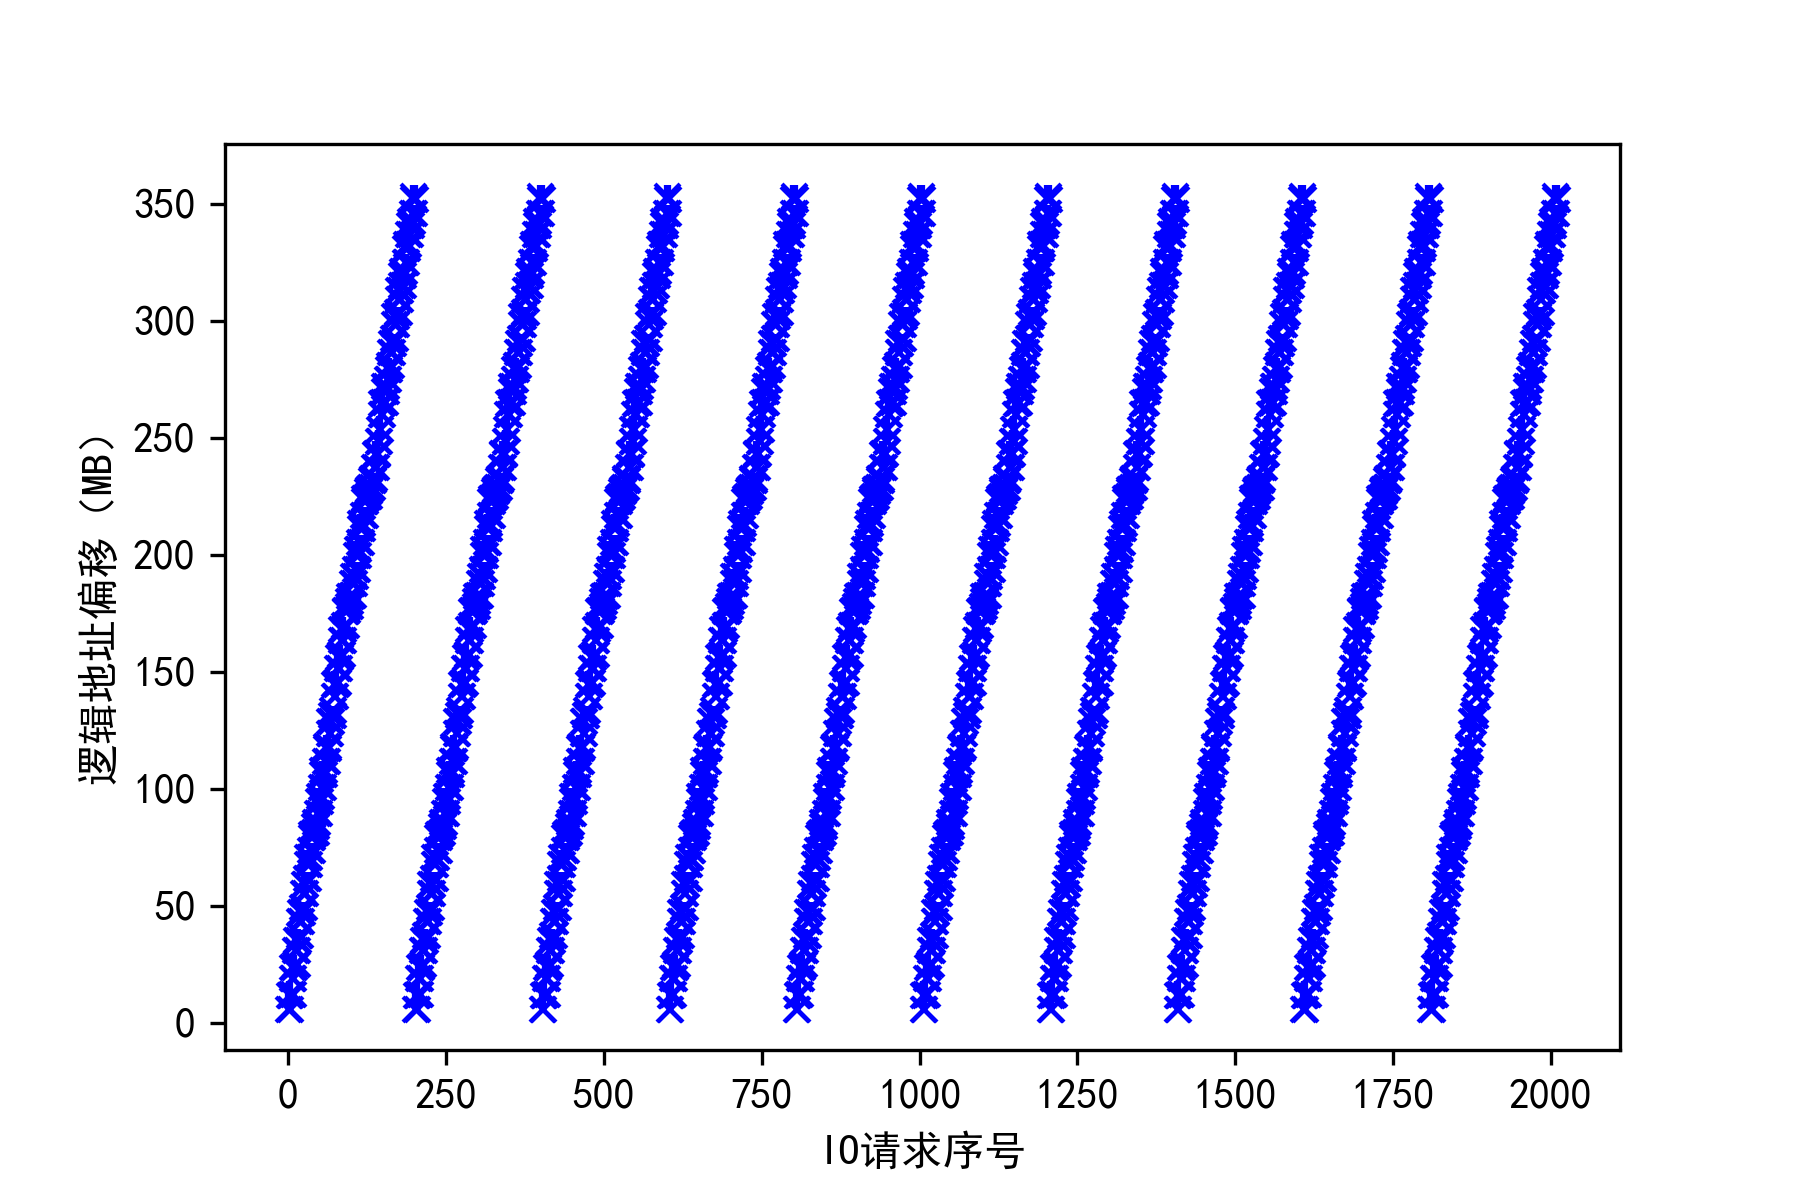
\includegraphics[width=0.4\textwidth]{iotrace_lammps.png}}
  \hspace{4em}
  \subcaptionbox{LAMMPS的IO Trace(部分)\label{fig:iotrace_lammps_sub}}
      {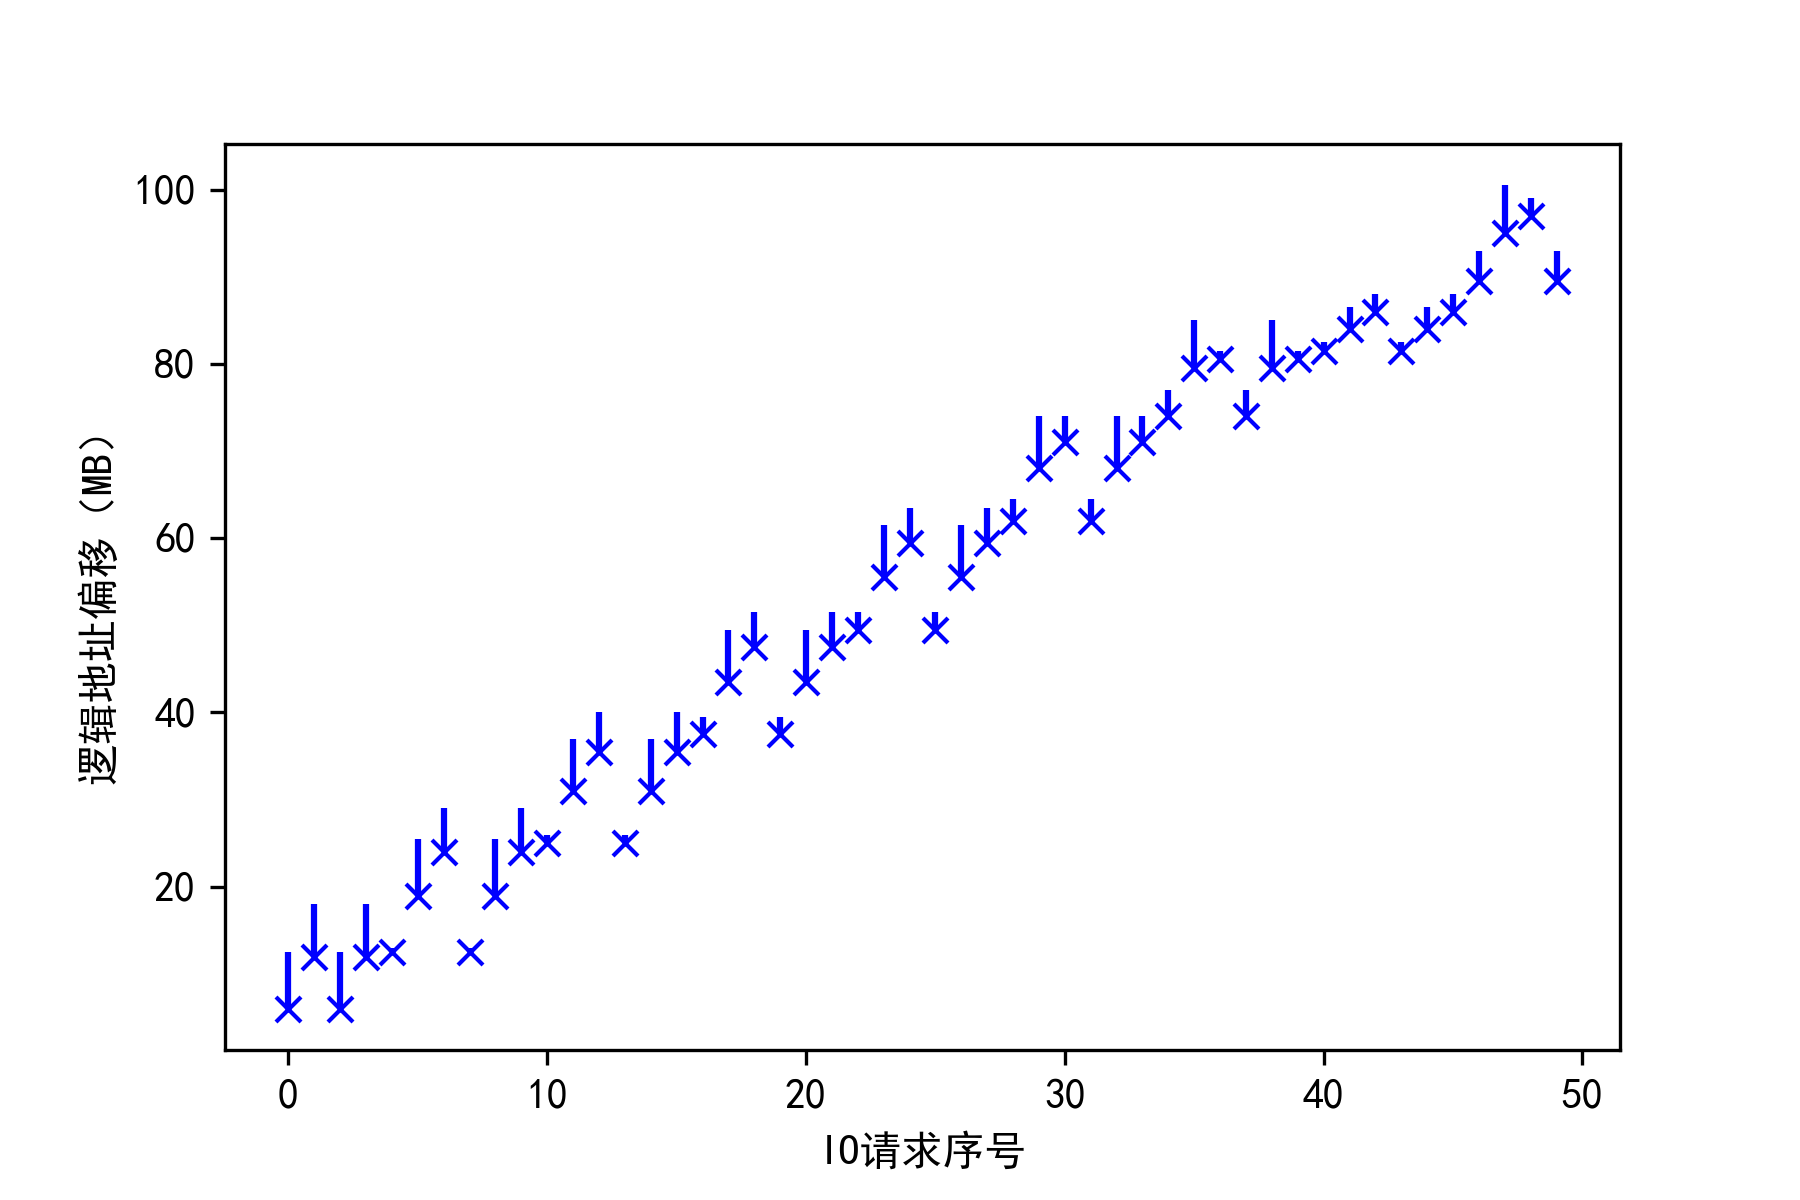
\includegraphics[width=0.4\textwidth]{iotrace_lammps_sub.png}}
  \caption{LAMMPS的IO Trace}
  \label{fig:iotrace_lammps_all}
\end{figure}

图\ref{fig:iotrace_lammps_all}展示了LAMMPS的IO Trace,采集到的IO Trace全部请求均为写请求。如图\ref{fig:iotrace_lammps},LAMMPS对逻辑地址范围0-358MB内的空间反复写入。图\ref{fig:iotrace_lammps_sub}为对其中一段IO Trace放大显示的结果,其中x表示IO请求的起始位置,铅直线覆盖部分表示IO请求涉及的逻辑地址空间。可以观察到LAMMPS对同一段空间进行了多次写操作。统计得到LAMMPS的这段IO Trace共写入了7075MB的数据,而访问的逻辑地址最大仅为358MB,显然这一过程中存在大量的覆盖写操作。

\begin{figure}[H]
  \centering
  \subcaptionbox{LAMMPS的IO请求数据量累积分布函数\label{fig:iotrace_lammps_iosize_cdf}}
    {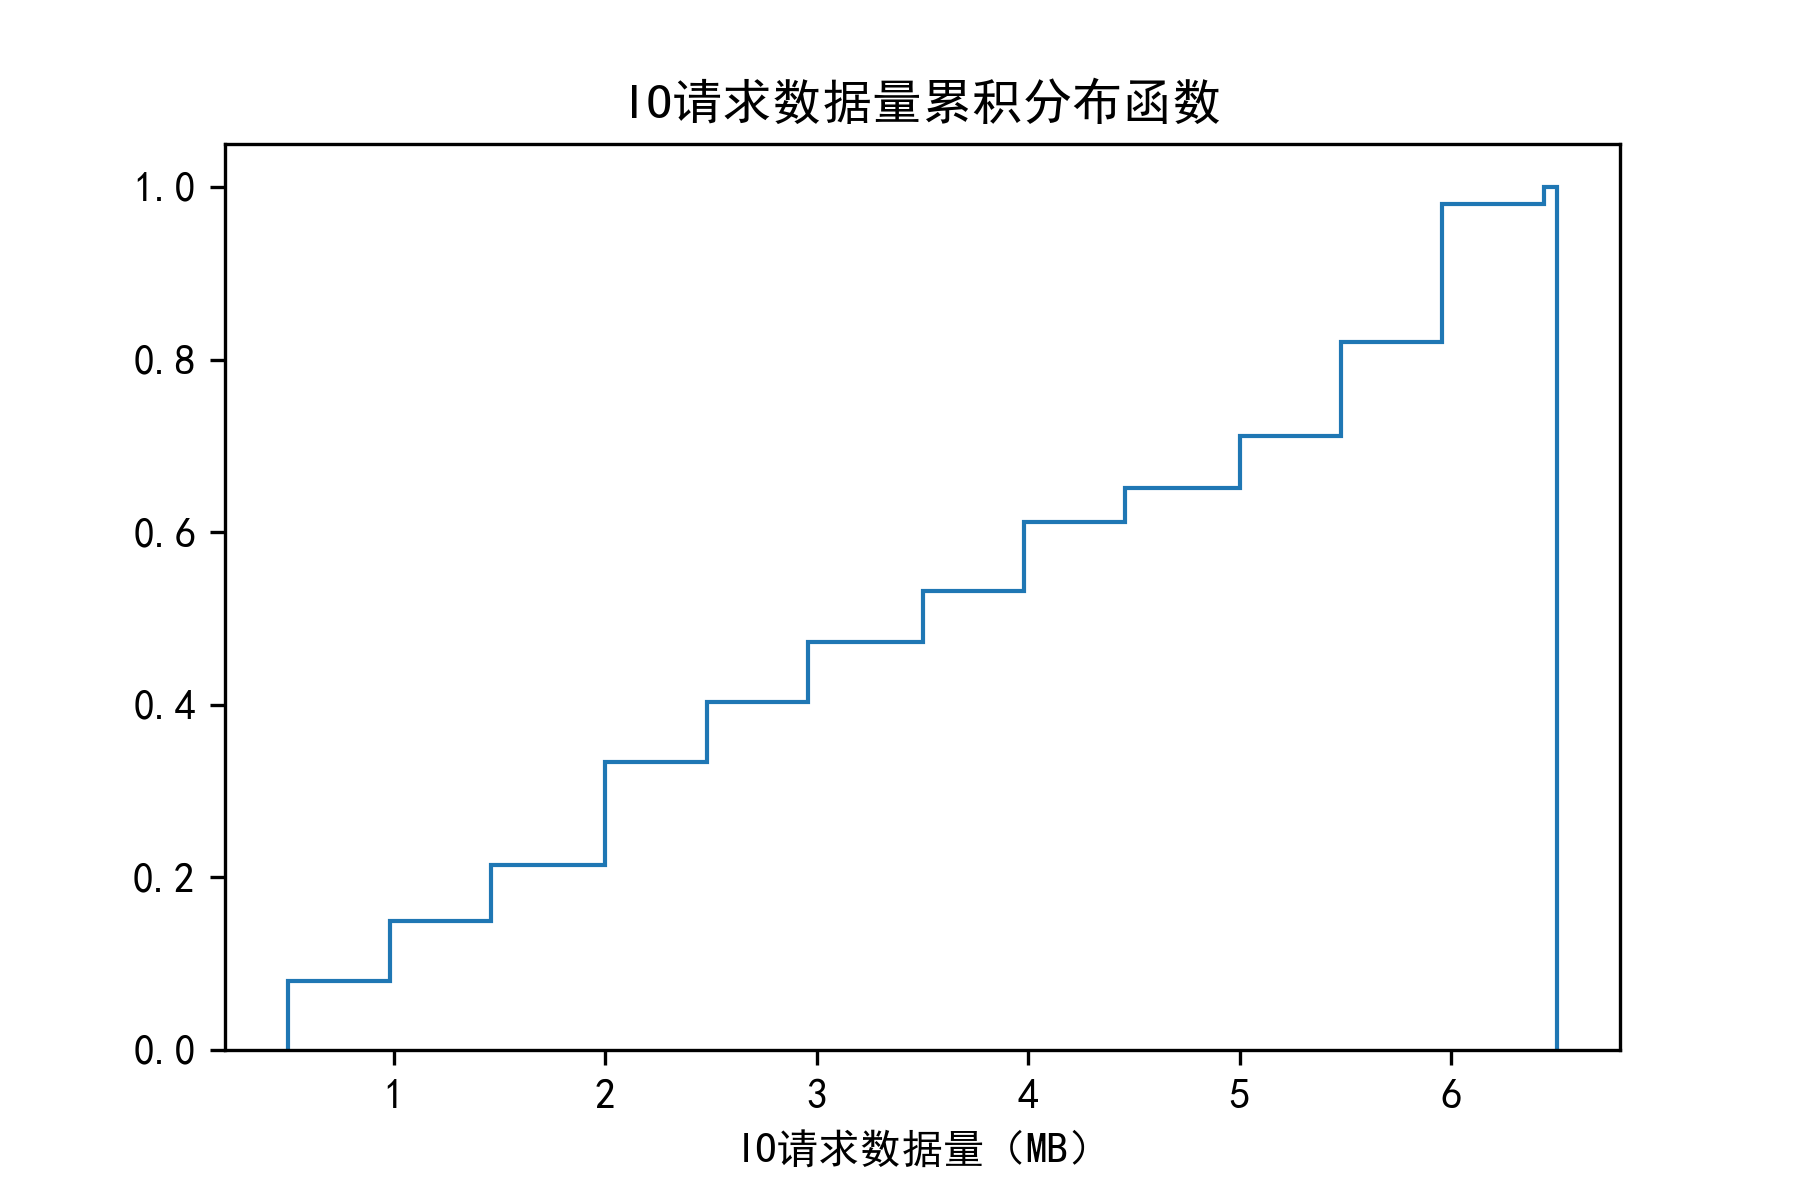
\includegraphics[width=0.25\textwidth]{iotrace_lammps_iosize_cdf.png}}
  \hspace{1em}
  \subcaptionbox{LAMMPS的IO请求起始地址页内偏移量累积分布函数\label{fig:iotrace_lammps_iostart_cdf}}
      {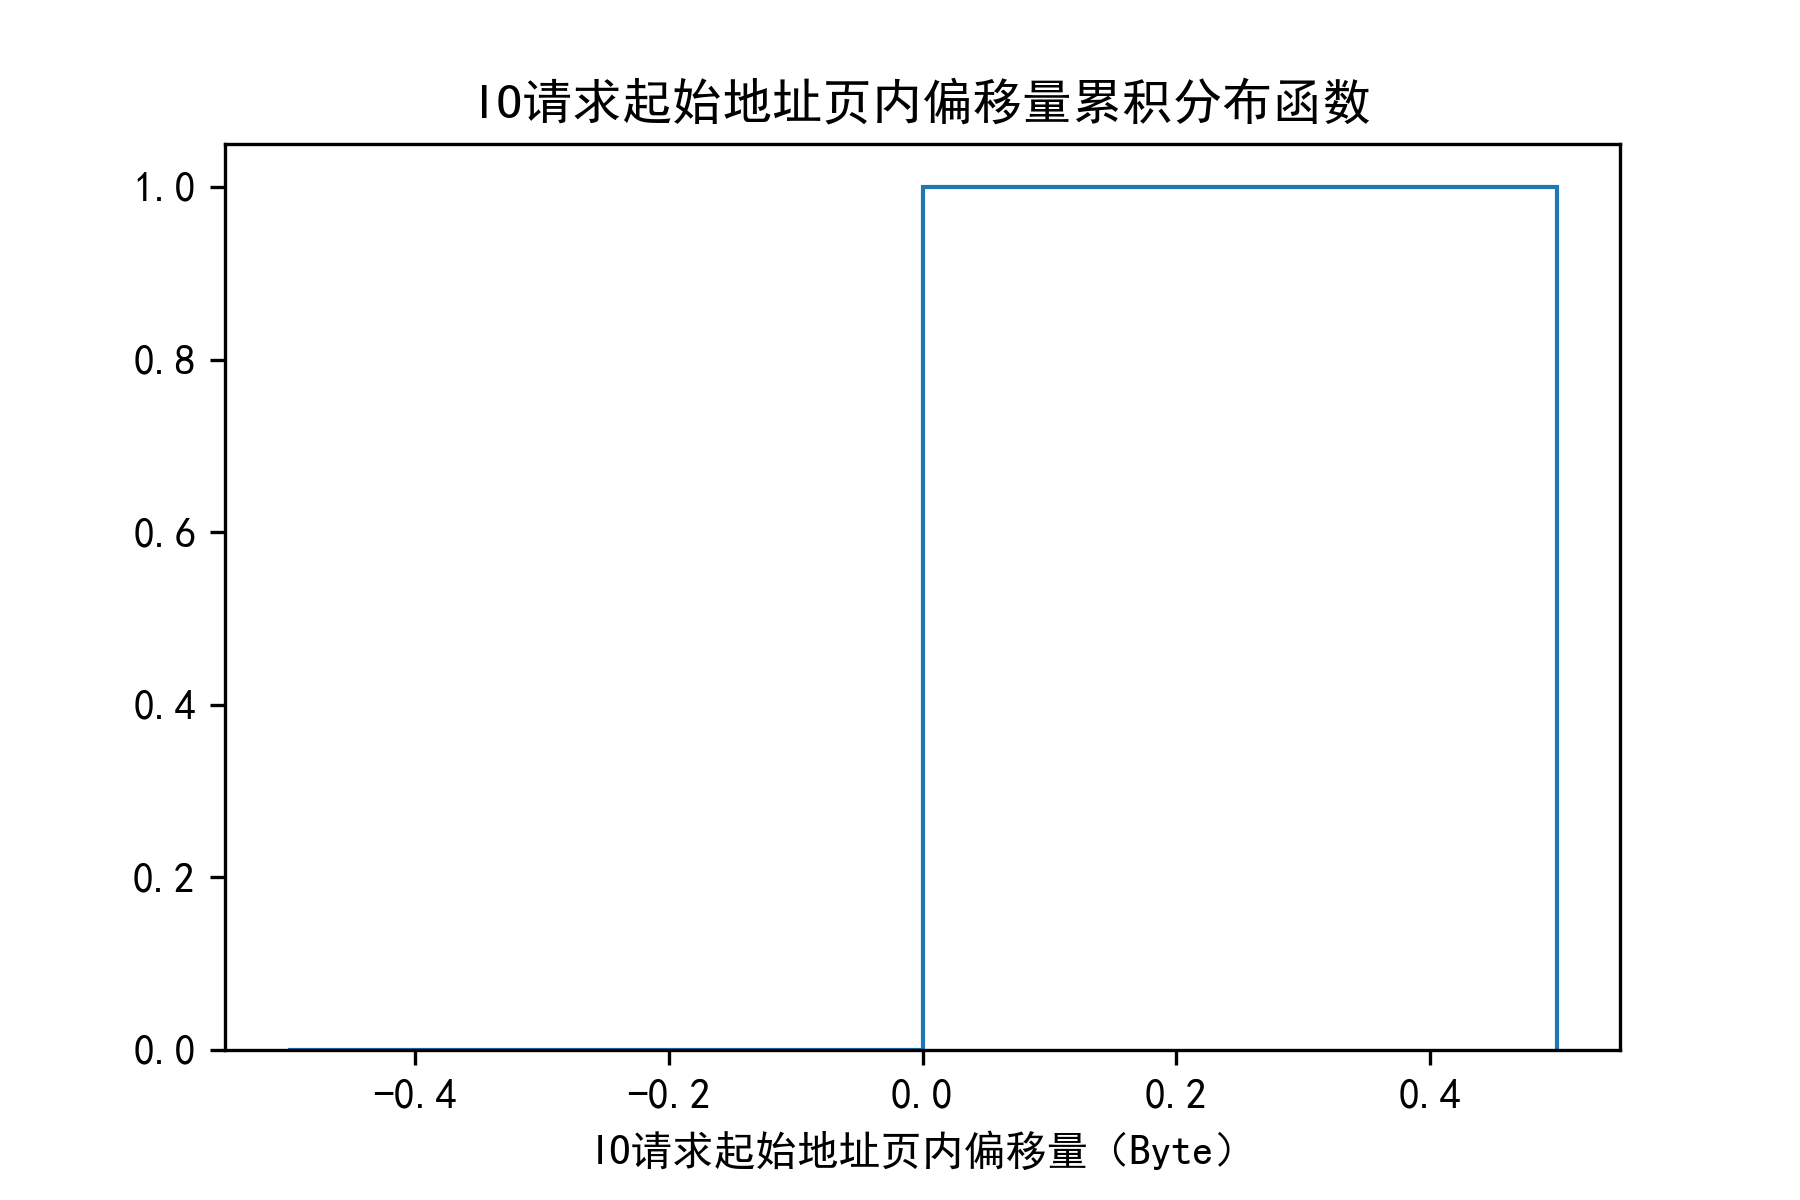
\includegraphics[width=0.25\textwidth]{iotrace_lammps_iostart_cdf.png}}
      \hspace{1em}
      \subcaptionbox{LAMMPS的IO请求结束地址页内偏移量累积分布函数\label{fig:iotrace_lammps_ioend_cdf}}
          {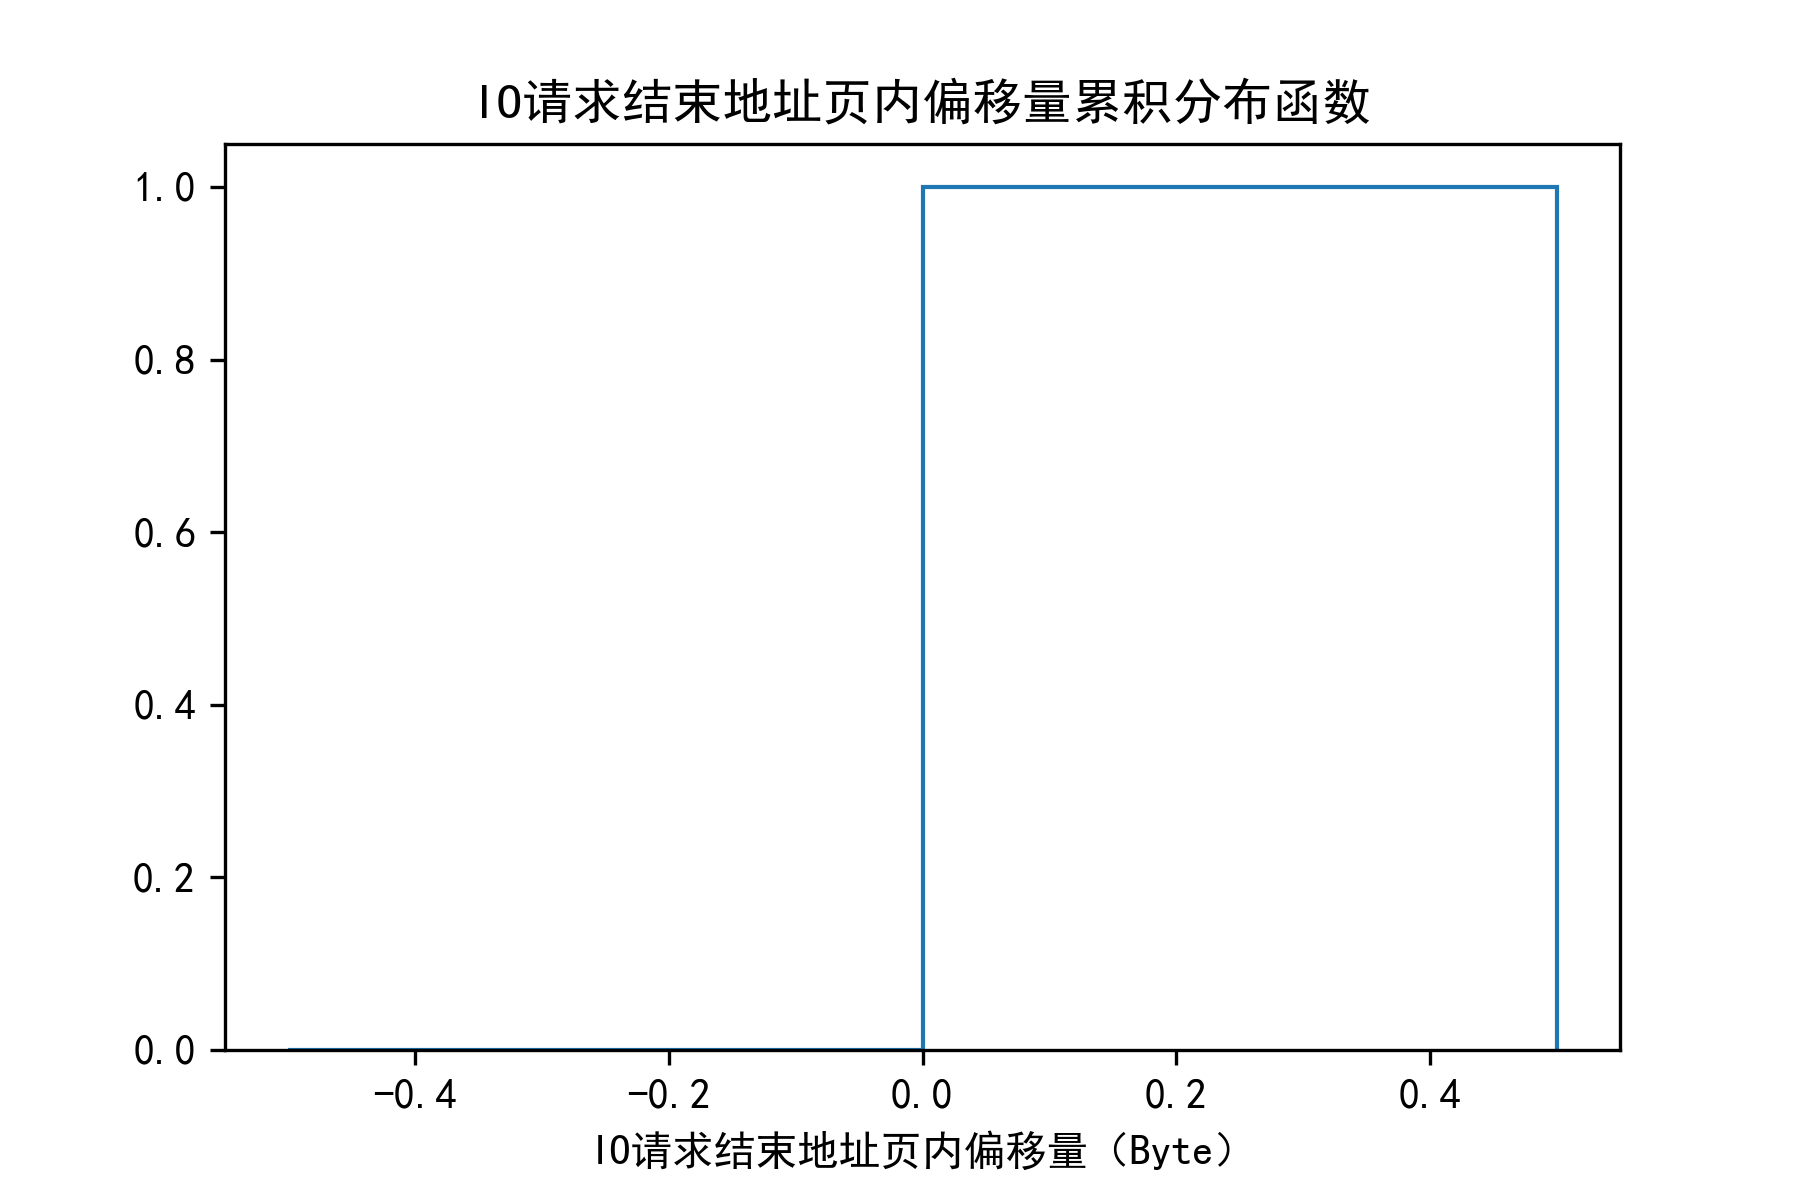
\includegraphics[width=0.25\textwidth]{iotrace_lammps_ioend_cdf.png}}
  \caption{LAMMPS的IO请求按页对齐情况}
  \label{fig:iotrace_lammps_iocdf}
\end{figure}
图\ref{fig:iotrace_lammps_iocdf}展示了LAMMPS的IO请求按页对齐的情况。这里的页大小取为后续实验使用的SSD页大小32768KB。如图\ref{fig:iotrace_lammps_iosize_cdf},几乎所有的IO请求大小都大于500KB。如图\ref{fig:iotrace_lammps_iostart_cdf}和图\ref{fig:iotrace_lammps_ioend_cdf},全部的IO请求起始地址和结束地址都对齐到页,同时表明IO请求的大小也按页对齐。

\begin{figure}[H]
  \centering
  \subcaptionbox{LAMMPS的IO请求起始地址块内偏移量累积分布函数\label{fig:iotrace_lammps_iostart_block_cdf}}
      {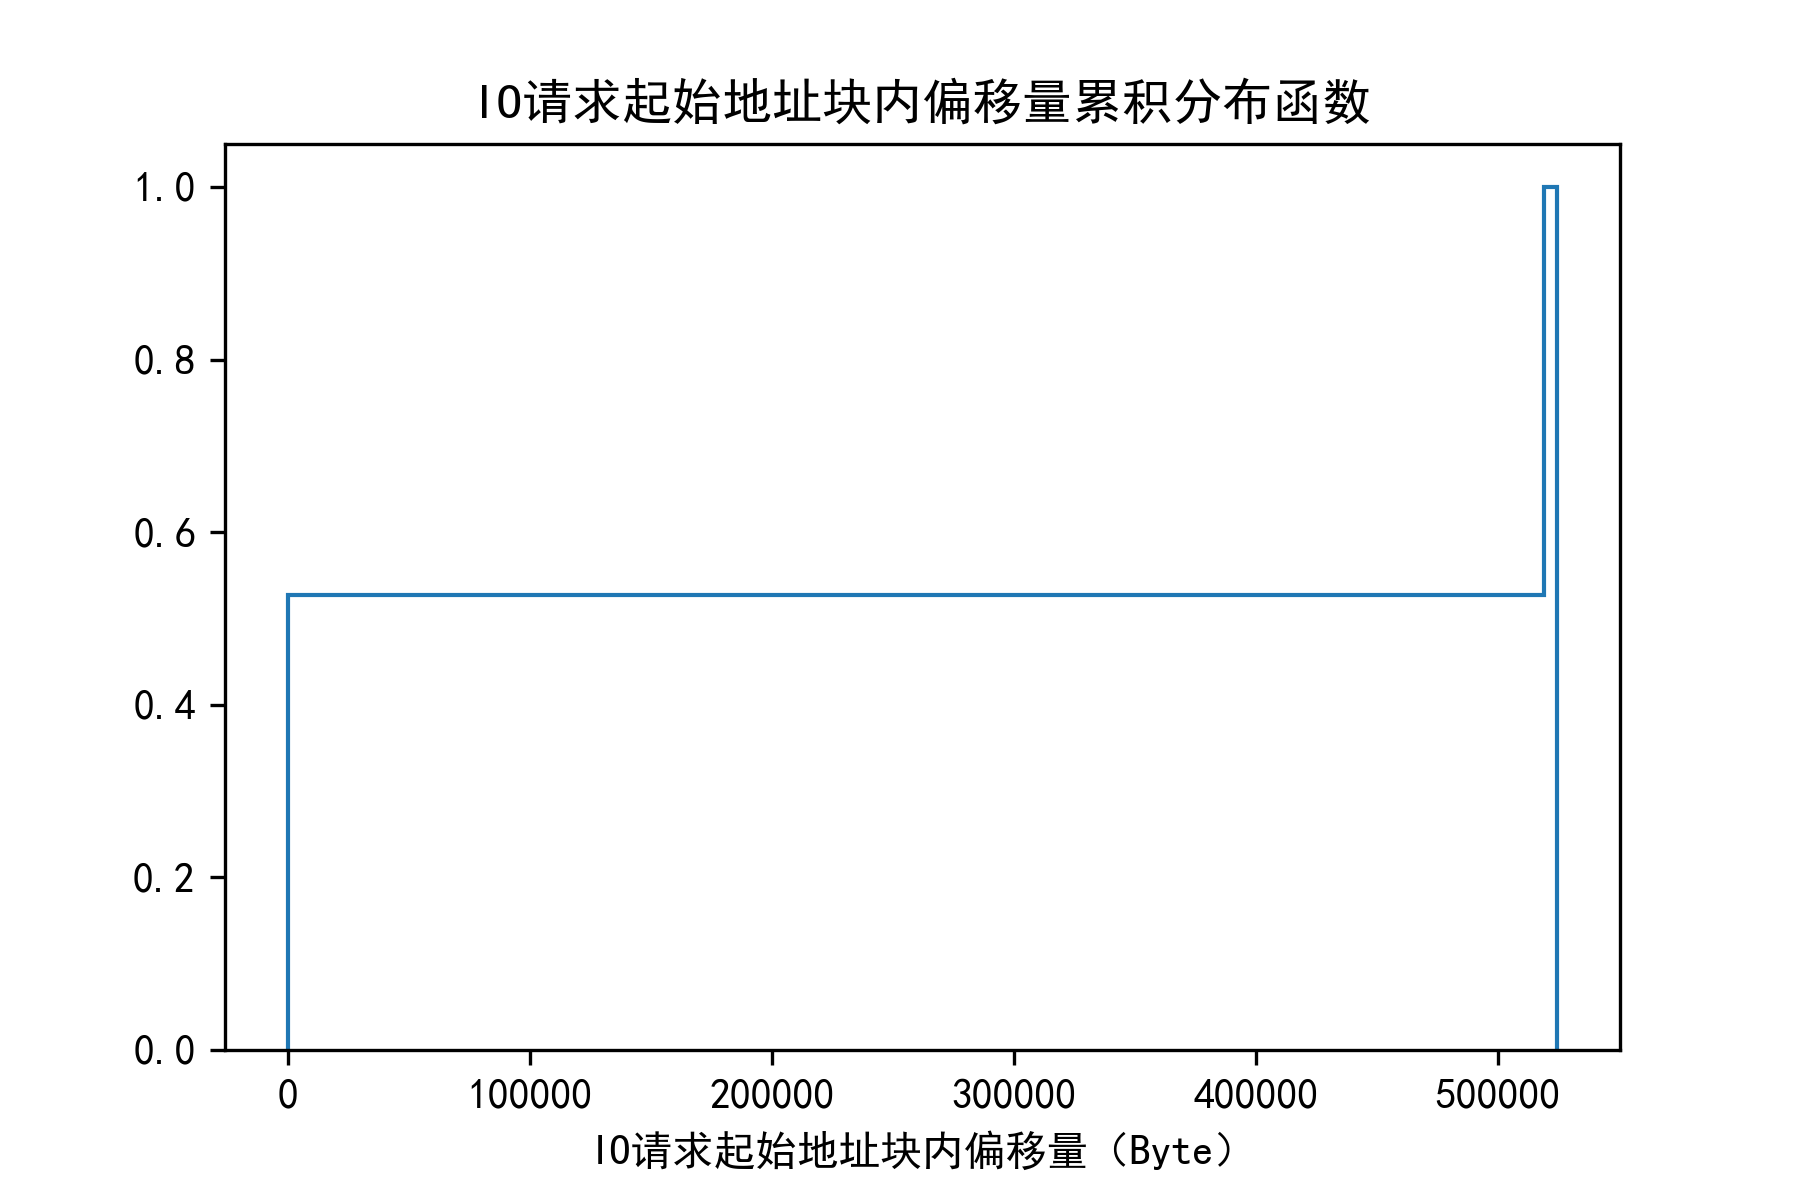
\includegraphics[width=0.4\textwidth]{iotrace_lammps_iostart_block_cdf.png}}
      \hspace{1em}
      \subcaptionbox{LAMMPS的IO请求结束地址块内偏移量累积分布函数\label{fig:iotrace_lammps_ioend_block_cdf}}
          {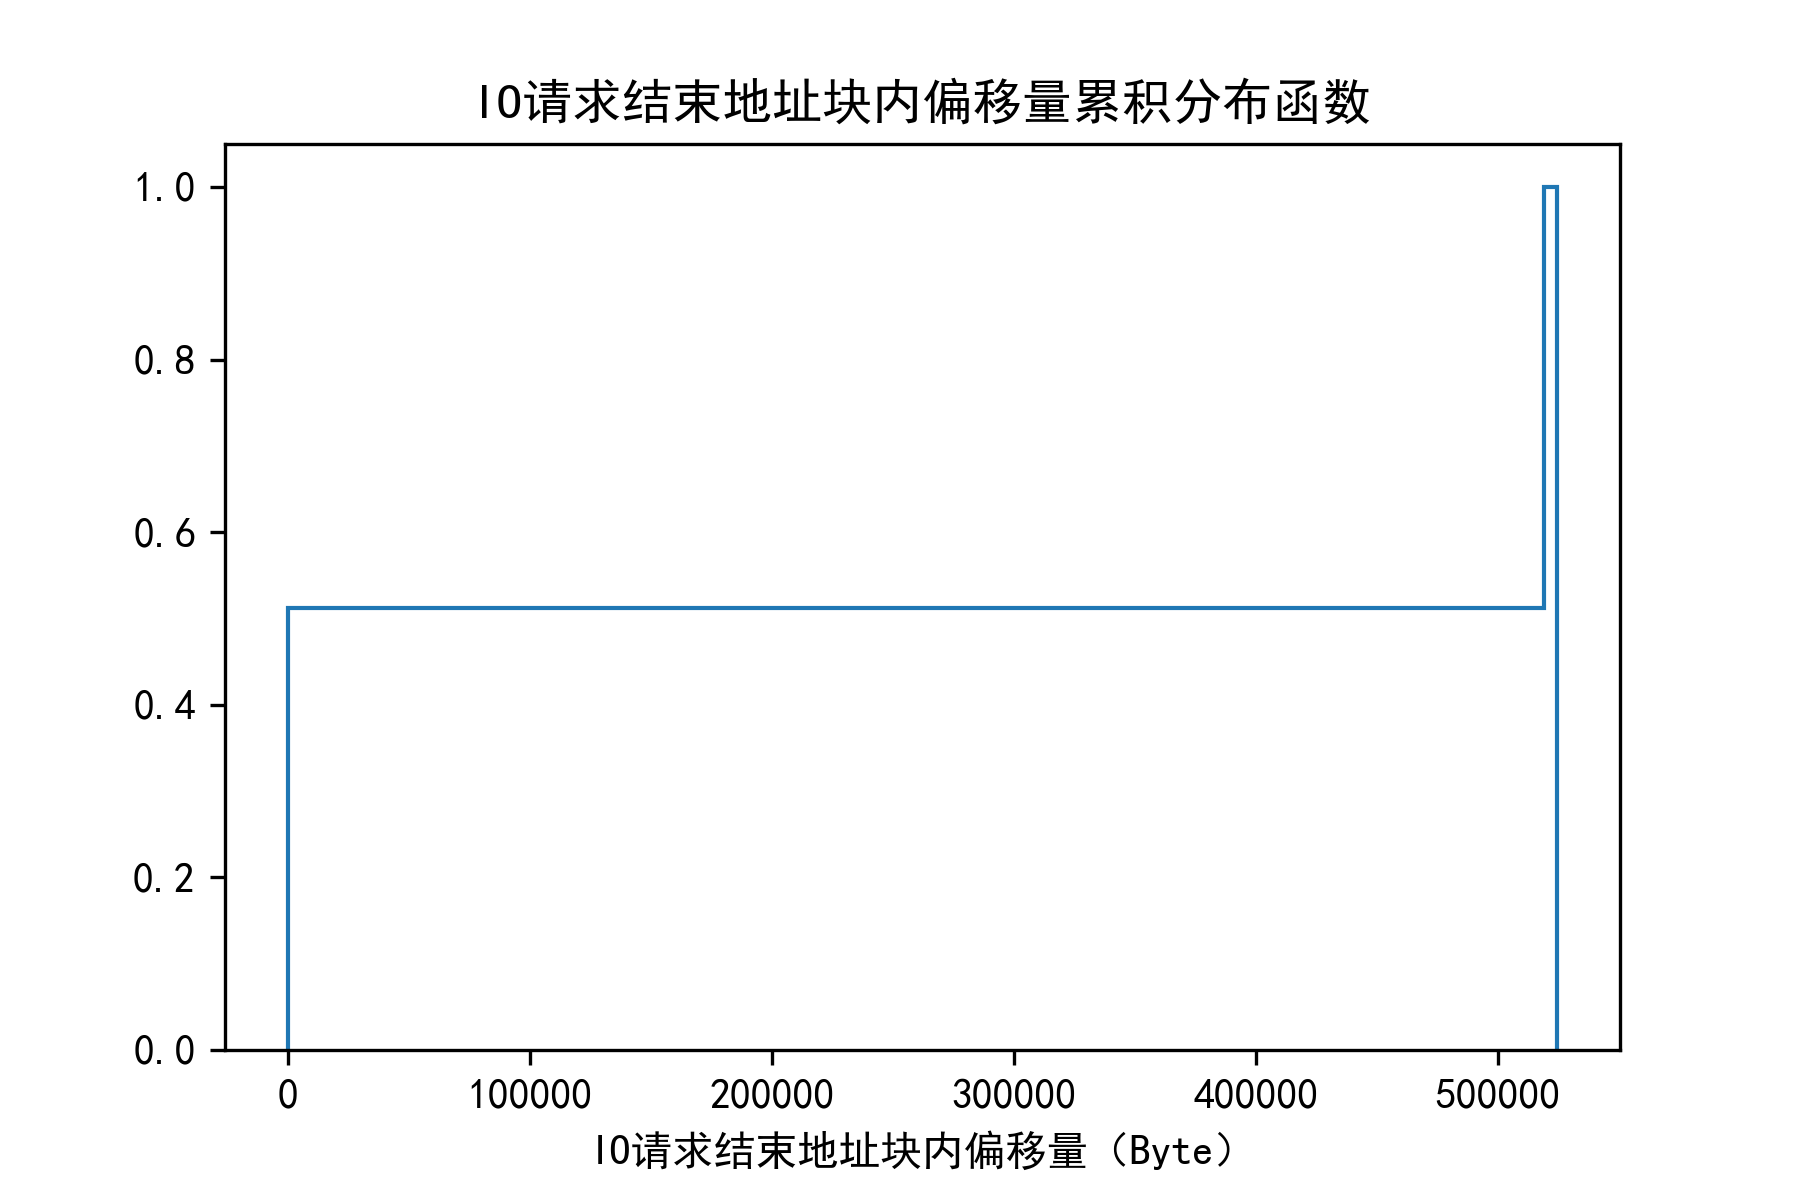
\includegraphics[width=0.4\textwidth]{iotrace_lammps_ioend_block_cdf.png}}
  \caption{LAMMPS的IO请求按块对齐情况}
  \label{fig:iotrace_lammps_iocdf_block}
\end{figure}

图\ref{fig:iotrace_lammps_iocdf_block}展示了LAMMPS的IO请求按块对齐的情况。这里的块大小取为后续实验使用的SSD块大小1MB(32个页)。由图\ref{fig:iotrace_lammps_iosize_cdf}知,约90\%的IO请求数据量均大于一个块。 如图\ref{fig:iotrace_lammps_iostart_block_cdf},大约半数的IO请求起始地址按块对齐,另一半IO请求的起始地址偏移为512KB,恰好为半个块大小。如图\ref{fig:iotrace_lammps_ioend_block_cdf},IO请求结束地址的情况与此类似。

\subsection{MACDRP应用的IO特征分析}
\label{ssc:ioana}
MACDRP能够模拟地震波在具有足够精度地表地形下的传播效果。
\begin{figure}[H]
  \centering
  \subcaptionbox{MACDRP的IO Trace\label{fig:iotrace_macdrp}}
    {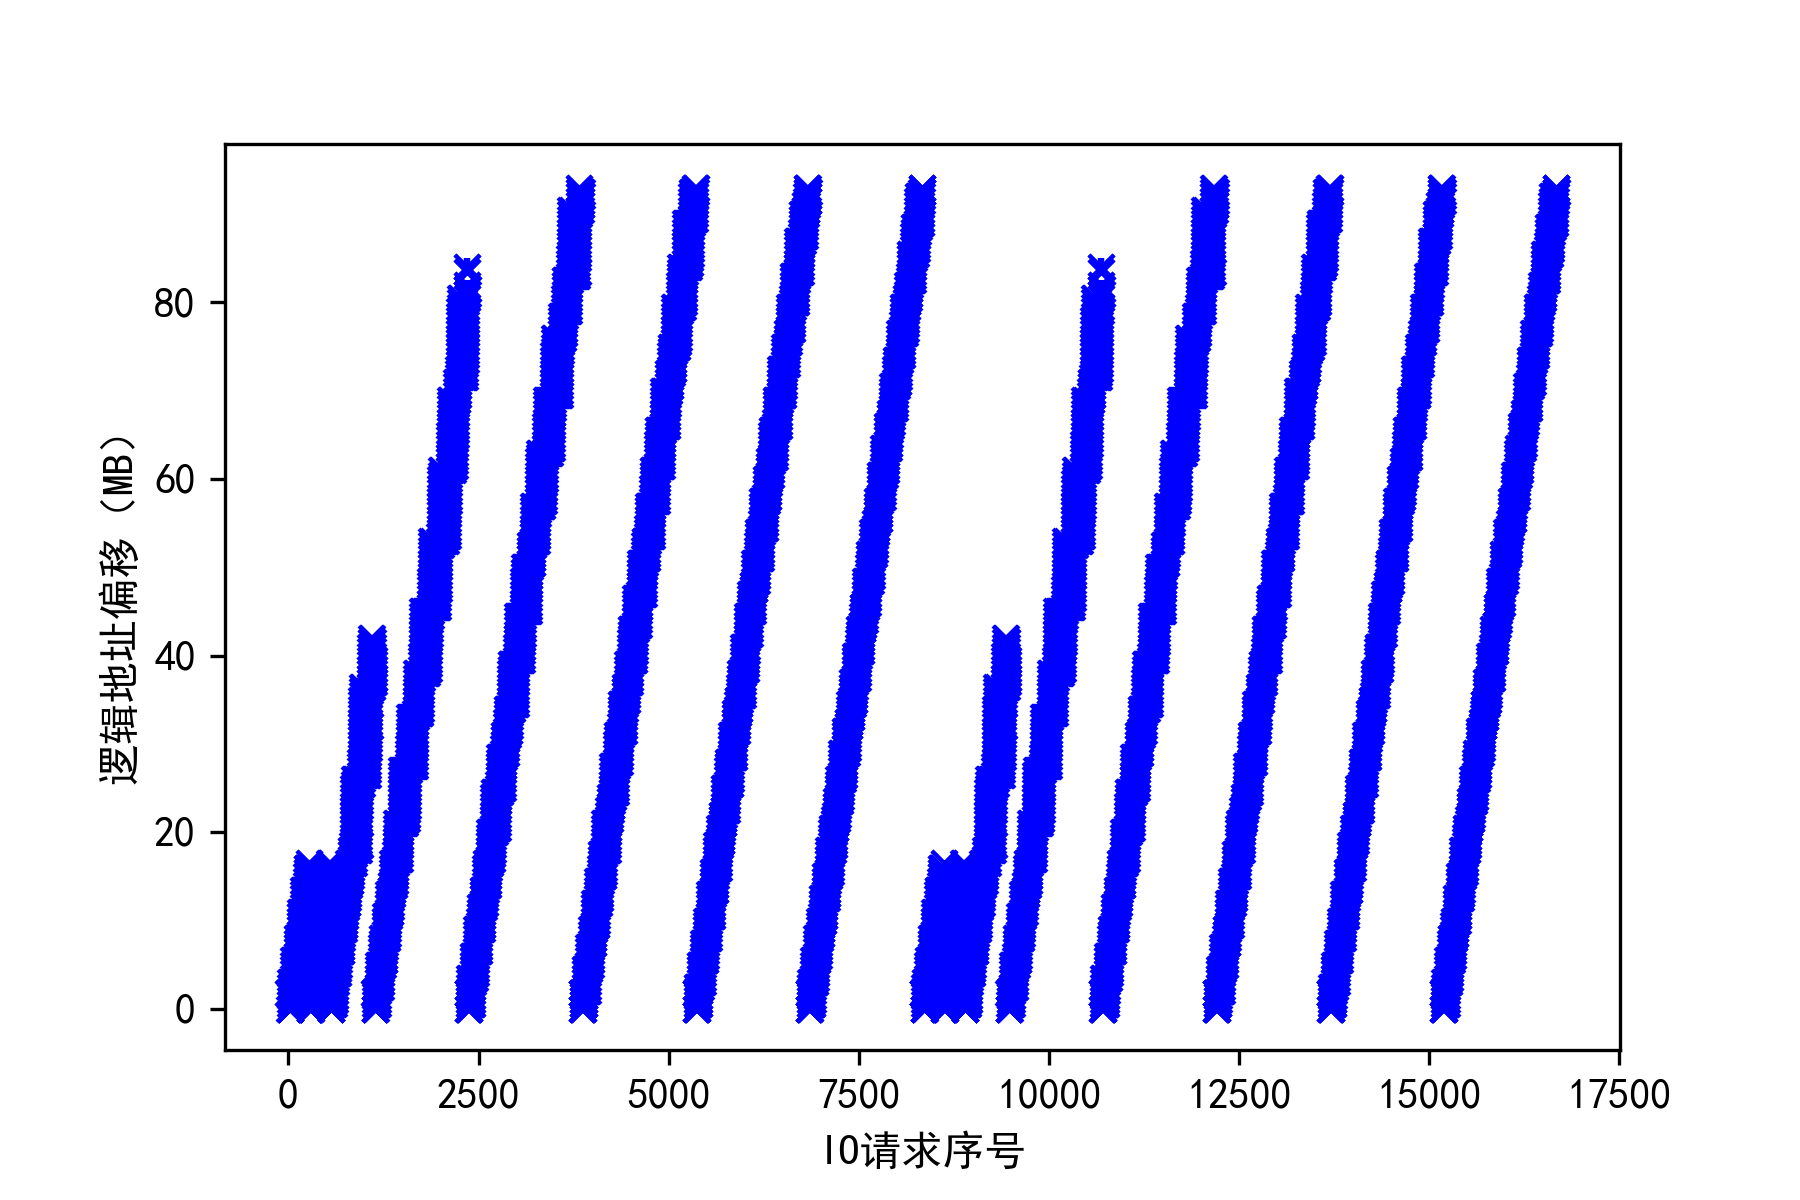
\includegraphics[width=0.4\textwidth]{iotrace_macdrp.png}}
  \hspace{4em}
  \subcaptionbox{MACDRP的IO Trace(部分)\label{fig:iotrace_macdrp_sub}}
      {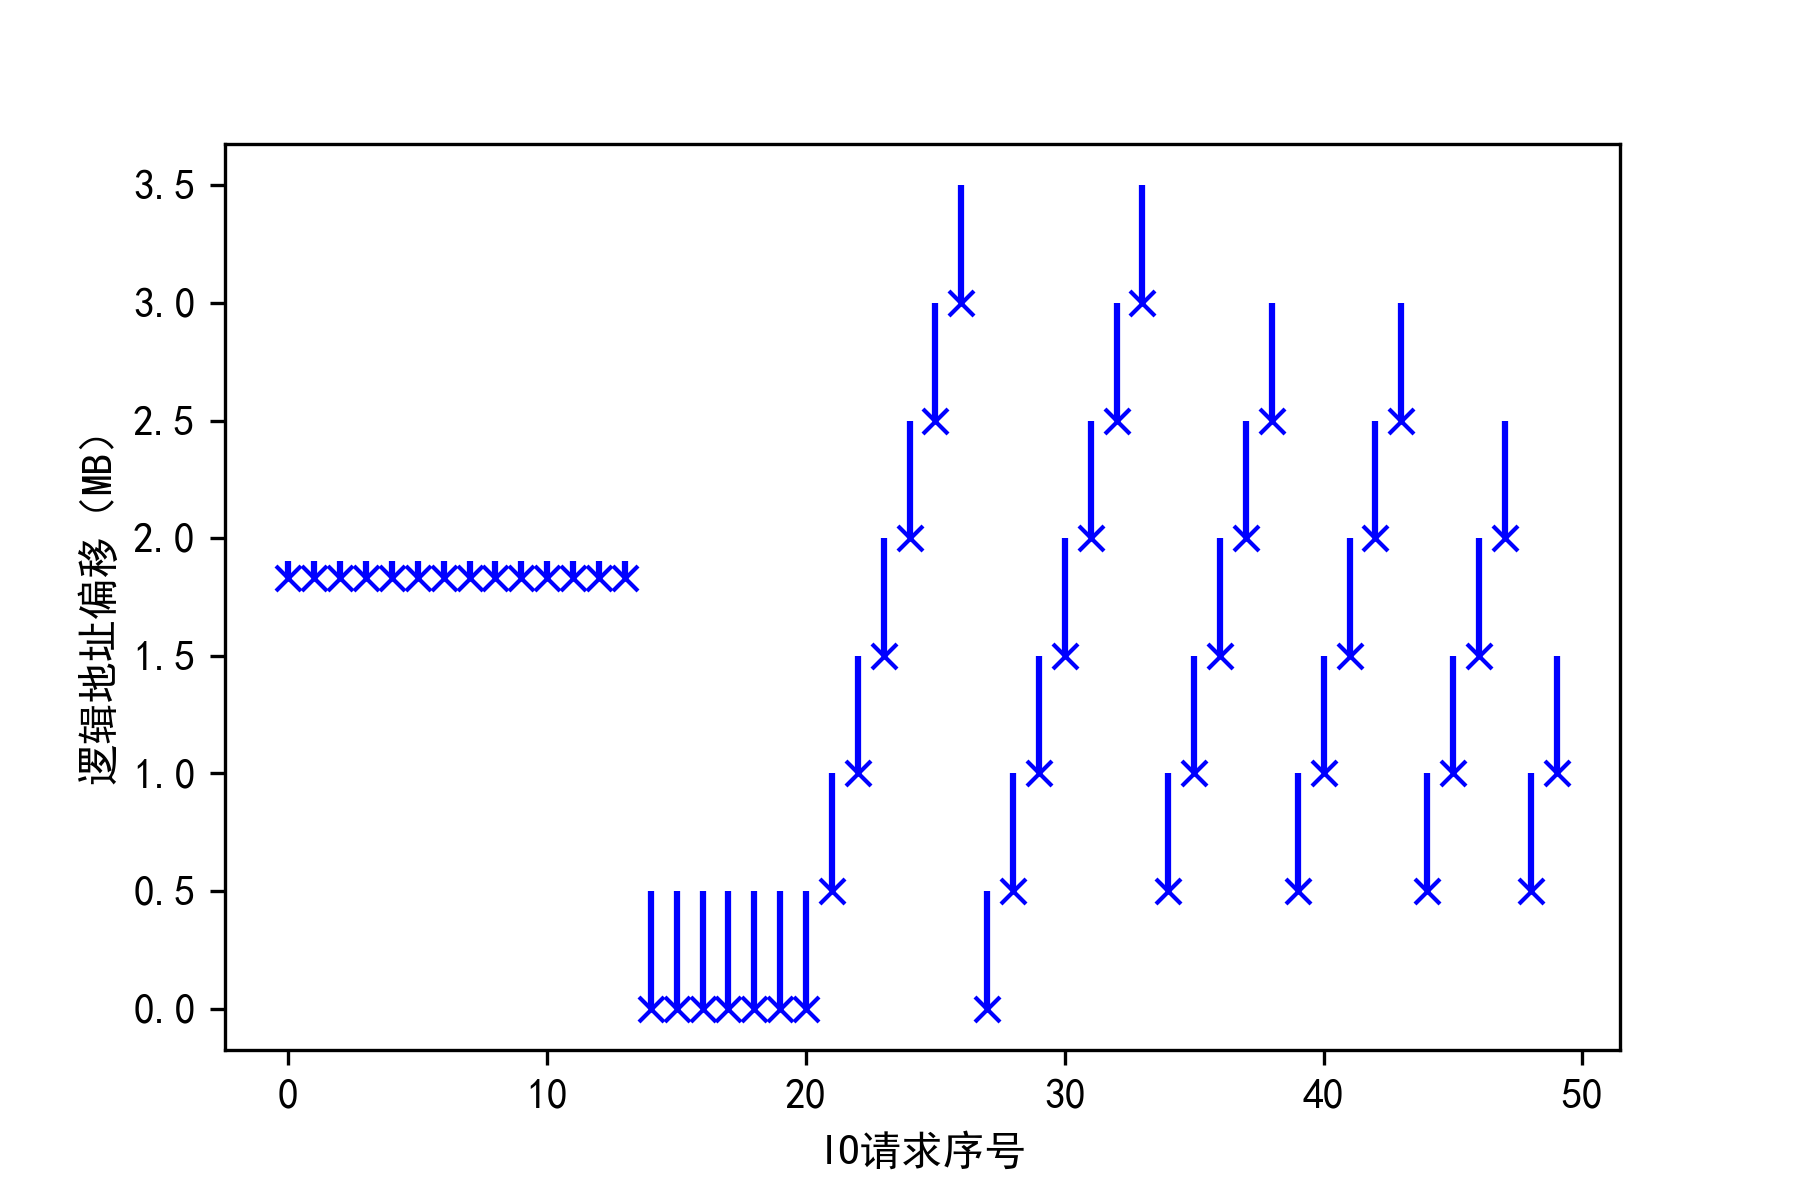
\includegraphics[width=0.4\textwidth]{iotrace_macdrp_sub.png}}
  \caption{MACDRP的IO Trace}
  \label{fig:iotrace_macdrp_all}
\end{figure}
图\ref{fig:iotrace_macdrp_all}展示了MACDRP的IO Trace,采集到的IO Trace全部请求均为写请求。与LAMMPS的情况类似,MACDRP同样在有限的逻辑地址空间内进行了大量覆盖写操作。如图\ref{fig:iotrace_macdrp},MACDRP在逻辑地址范围0-93MB内的空间反复写入了高达8256MB的数据。图\ref{fig:iotrace_macdrp_sub}为对其中一段IO Trace放大显示的结果,符号含义与图\ref{fig:iotrace_lammps_sub}相同。可以观察到MACDRP对同一段空间进行了高达7次写操作。这一过程中覆盖写的比例比LAMMPS更高。

\begin{figure}[H]
  \centering
  \subcaptionbox{MACDRP的IO请求数据量累积分布函数\label{fig:iotrace_macdrp_iosize_cdf}}
    {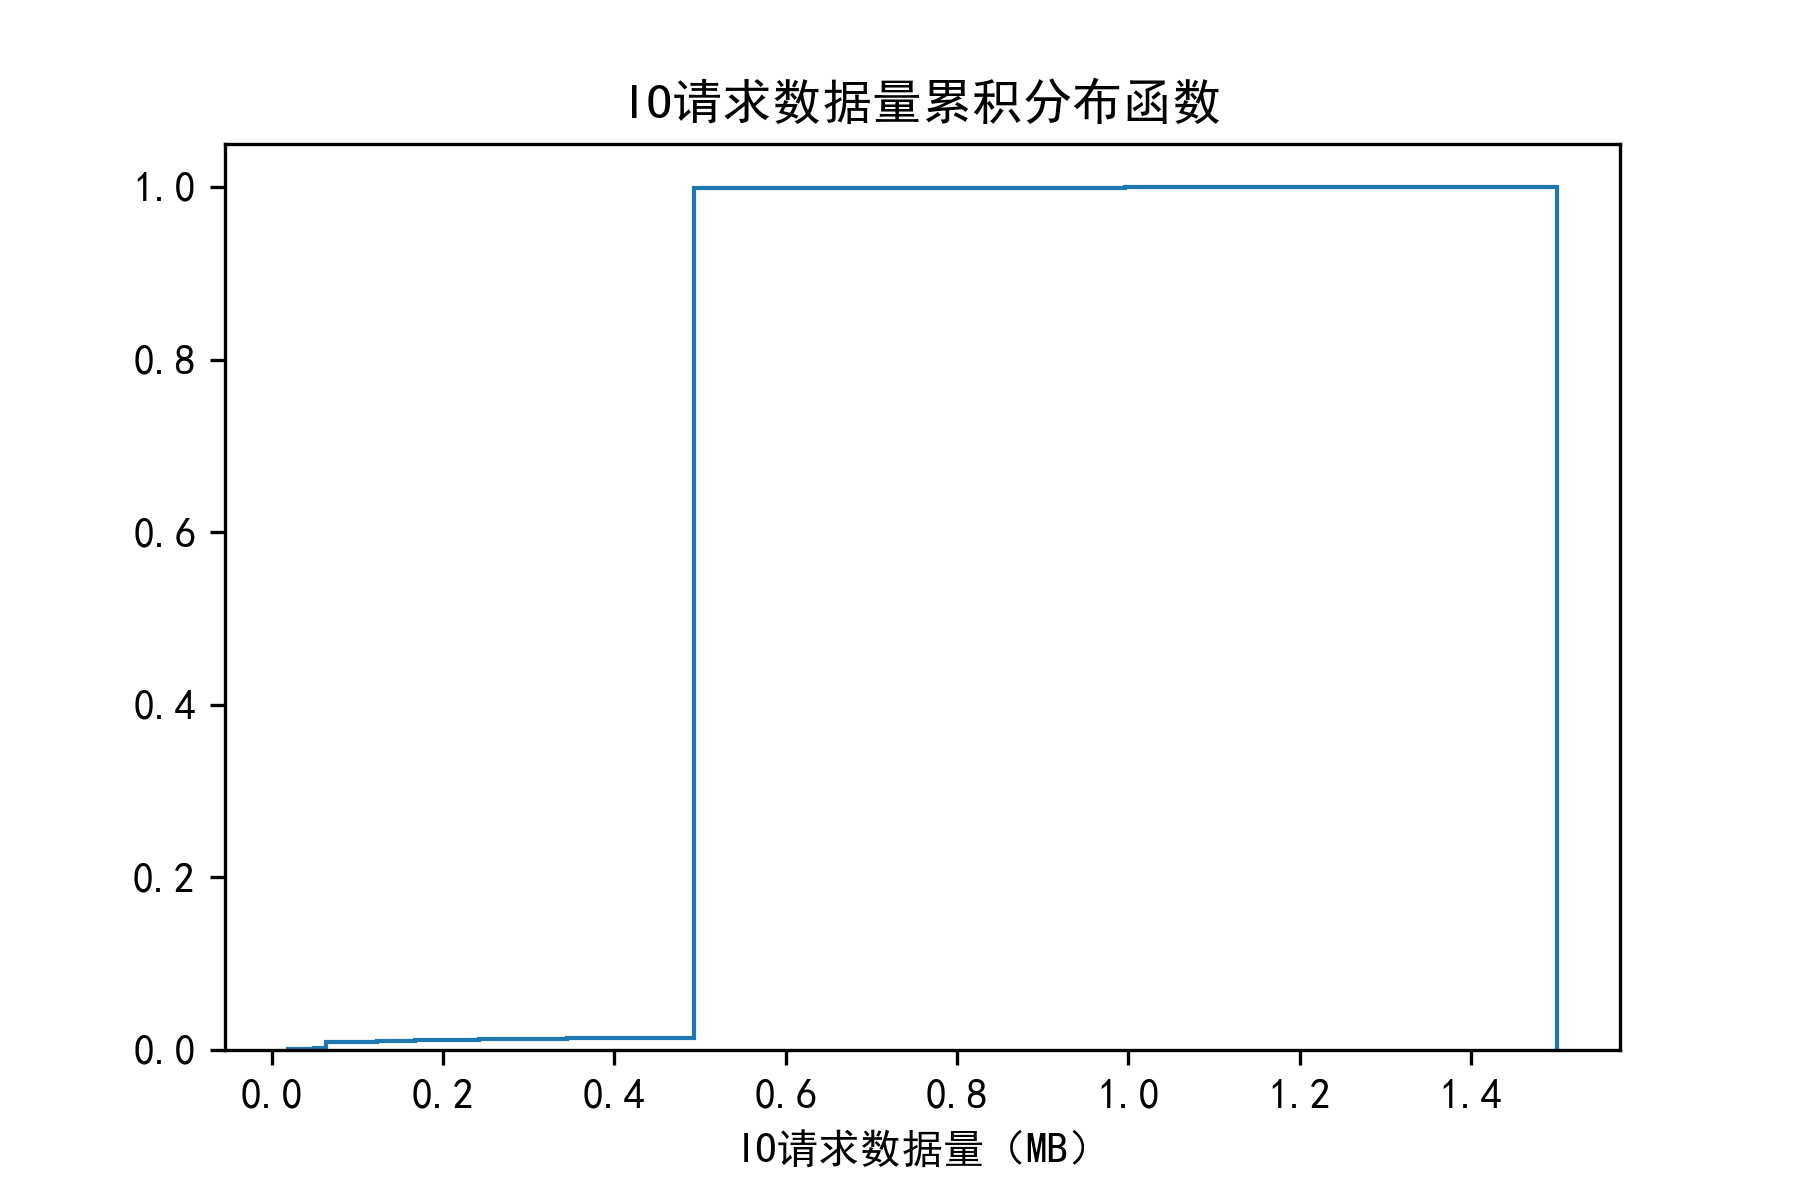
\includegraphics[width=0.25\textwidth]{iotrace_macdrp_iosize_cdf.png}}
  \hspace{1em}
  \subcaptionbox{MACDRP的IO请求起始地址页内偏移量累积分布函数\label{fig:iotrace_macdrp_iostart_cdf}}
      {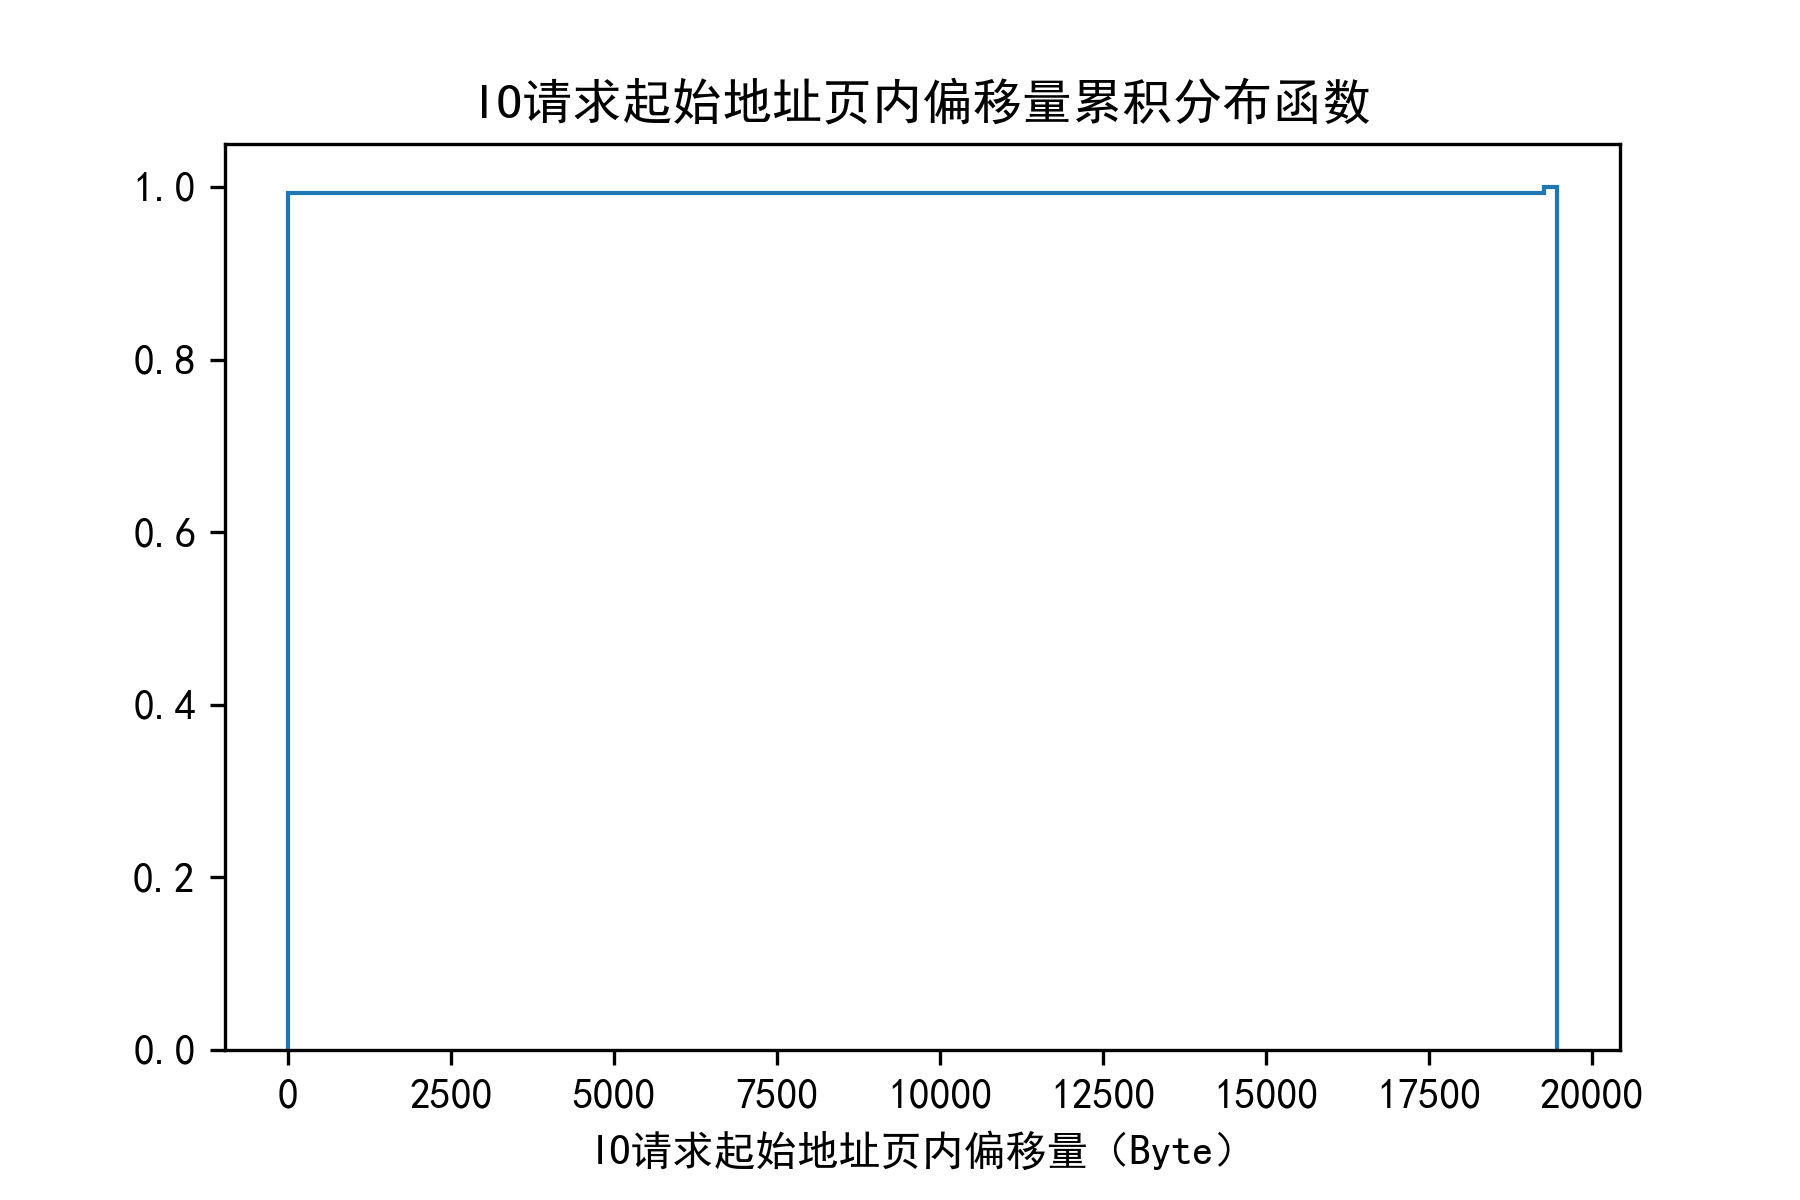
\includegraphics[width=0.25\textwidth]{iotrace_macdrp_iostart_cdf.png}}
      \hspace{1em}
      \subcaptionbox{MACDRP的IO请求结束地址页内偏移量累积分布函数\label{fig:iotrace_macdrp_ioend_cdf}}
          {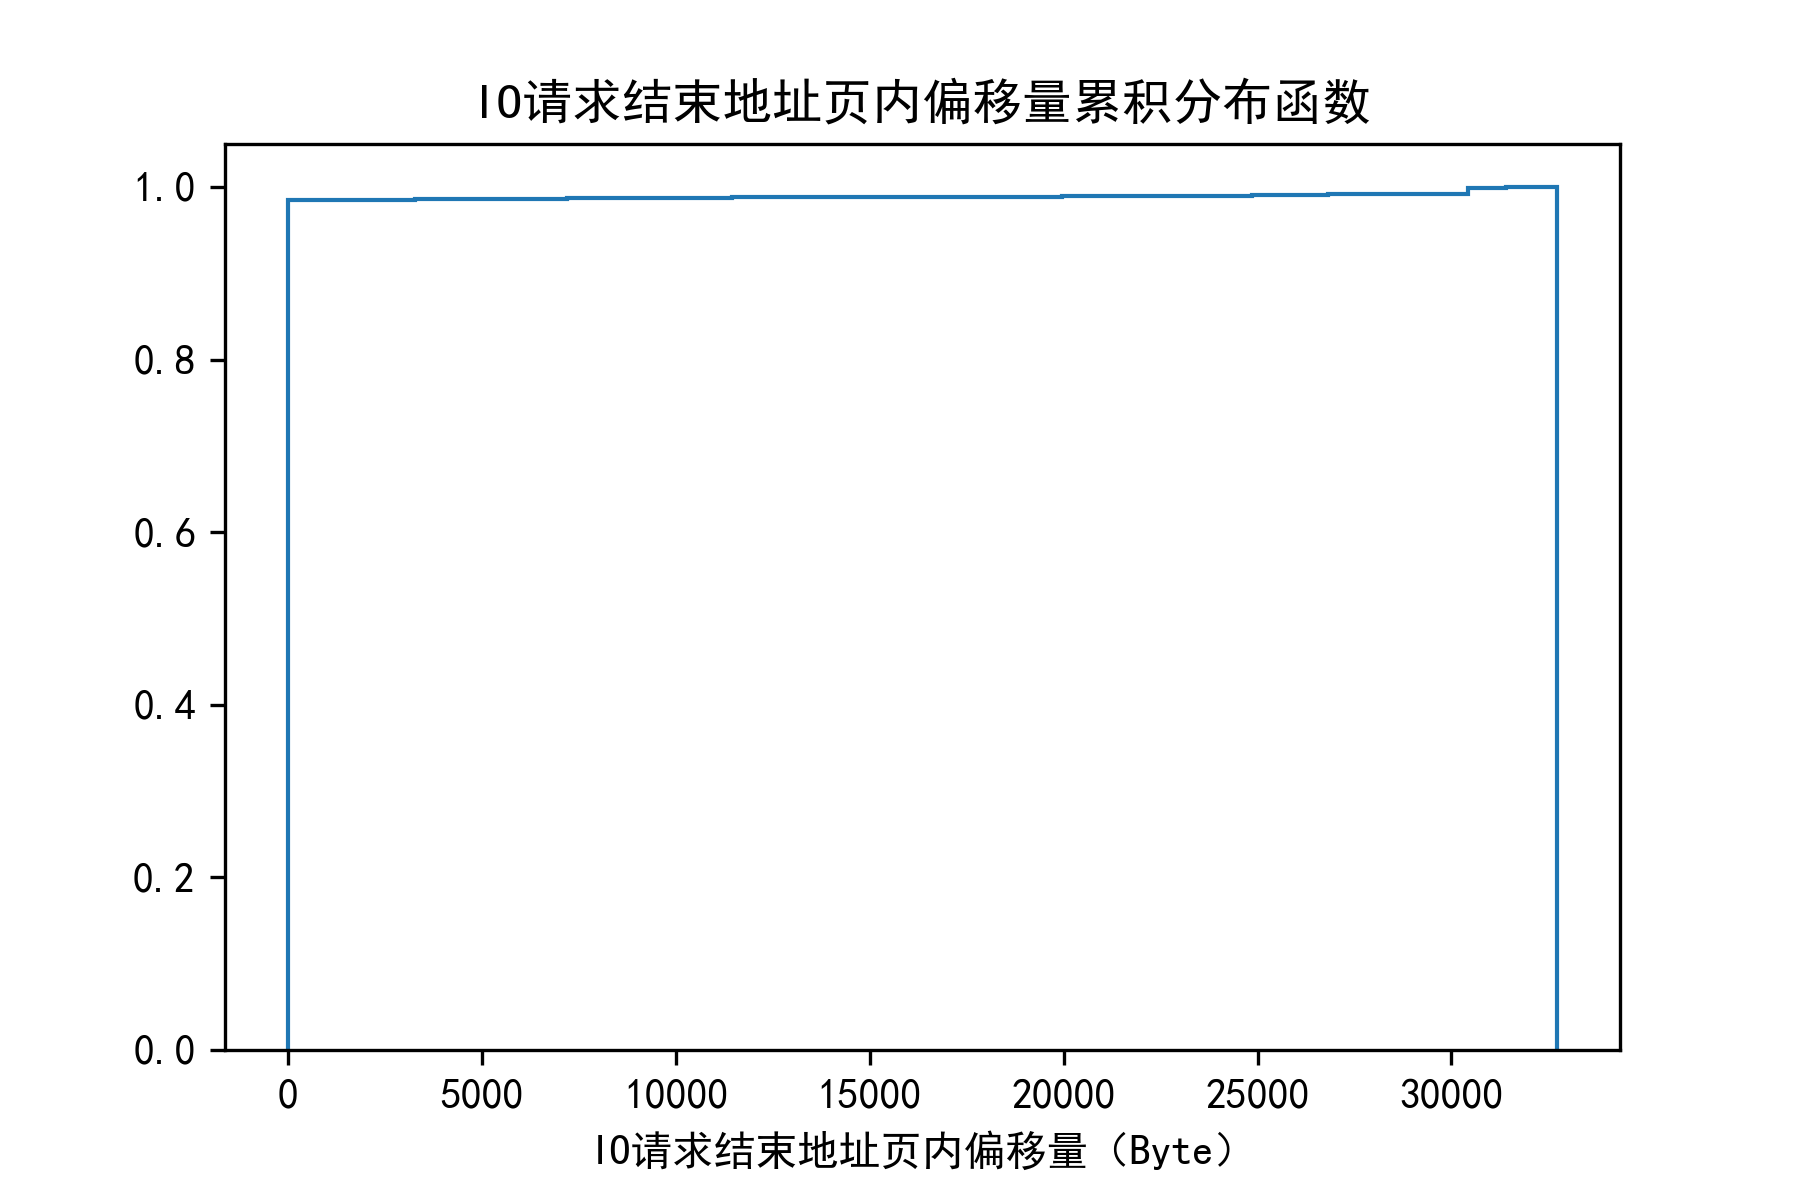
\includegraphics[width=0.25\textwidth]{iotrace_macdrp_ioend_cdf.png}}
  \caption{MACDRP的IO请求按页对齐情况}
  \label{fig:iotrace_macdrp_iocdf}
\end{figure}

图\ref{fig:iotrace_macdrp_iocdf}显示了MACDRP的IO请求按页对齐的情况。由图\ref{fig:iotrace_macdrp_iostart_cdf}和图\ref{fig:iotrace_macdrp_ioend_cdf}可知,其绝大部分IO请求都能按页对齐,仅有少量请求的开始/结束地址页内偏移量不为0。图\ref{fig:iotrace_macdrp_iosize_cdf}表明MACDRP的几乎所有IO请求数据量大小均相同,为512KB。

\begin{figure}[H]
  \centering
  \subcaptionbox{MACDRP的IO请求起始地址块内偏移量累积分布函数\label{fig:iotrace_macdrp_iostart_block_cdf}}
      {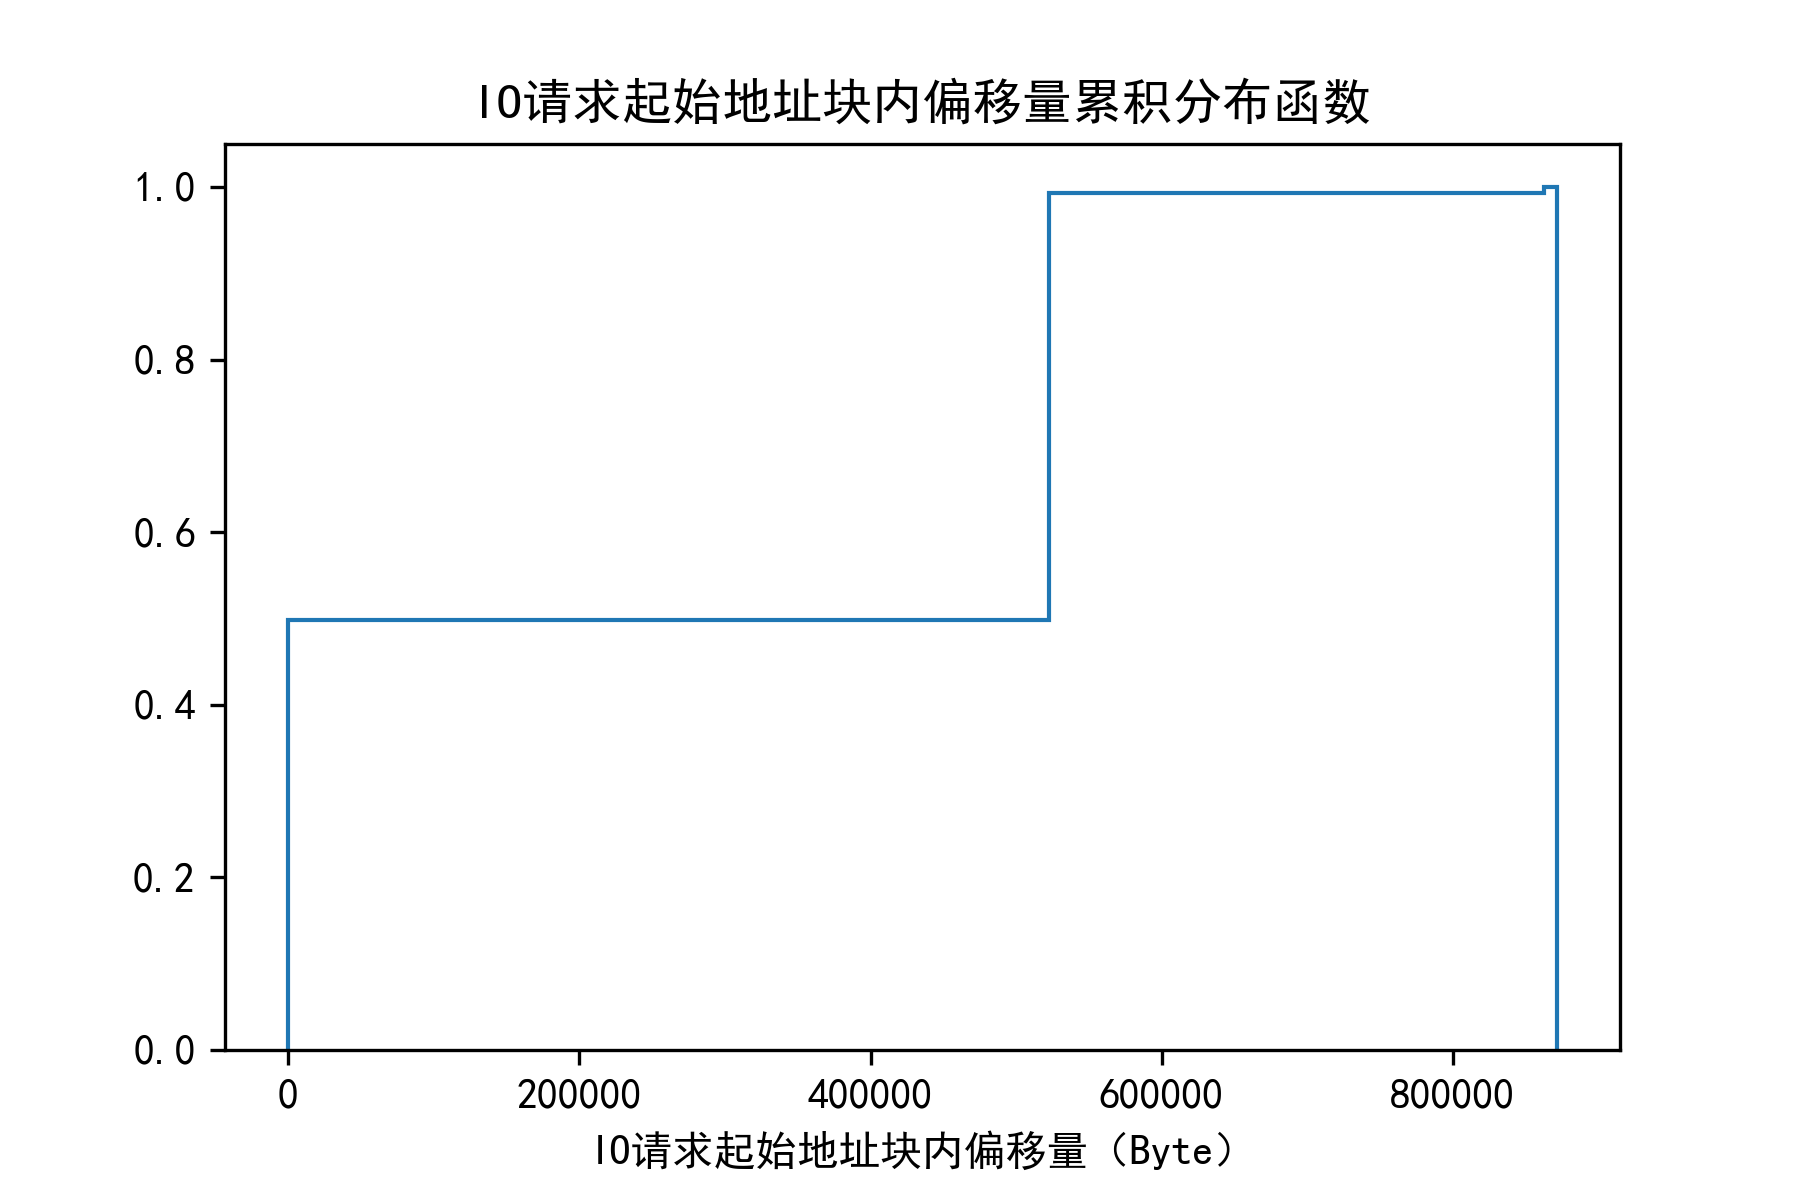
\includegraphics[width=0.4\textwidth]{iotrace_macdrp_iostart_block_cdf.png}}
      \hspace{1em}
      \subcaptionbox{MACDRP的IO请求结束地址块内偏移量累积分布函数\label{fig:iotrace_macdrp_ioend_block_cdf}}
          {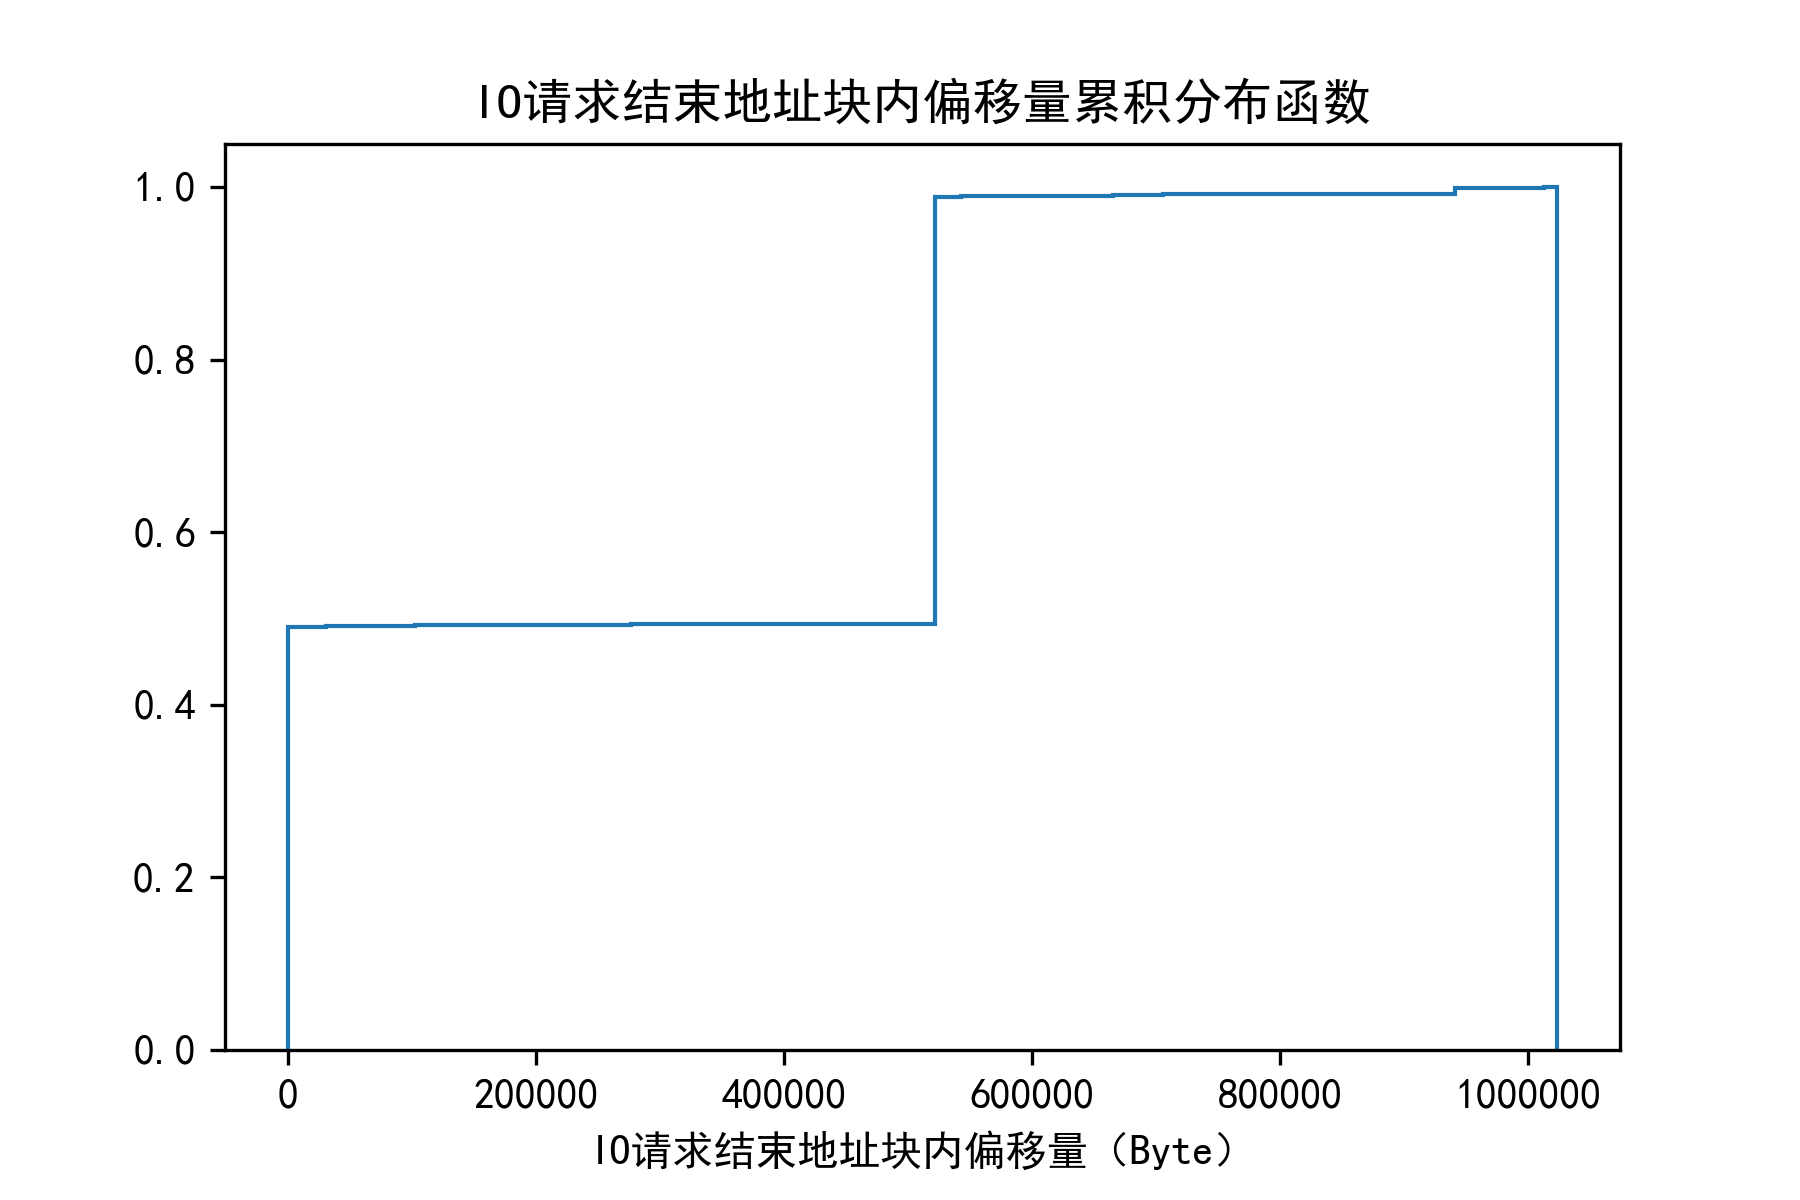
\includegraphics[width=0.4\textwidth]{iotrace_macdrp_ioend_block_cdf.png}}
  \caption{MACDRP的IO请求按块对齐情况}
  \label{fig:iotrace_macdrp_iocdf_block}
\end{figure}

图\ref{fig:iotrace_macdrp_iocdf_block}展示了MACDRP的IO请求按块对齐的情况。这里的块大小取为后续实验使用的SSD块大小1MB(32个页)。由图\ref{fig:iotrace_macdrp_iosize_cdf}知,几乎所有的IO请求数据量均为512KB,为半个块大小。 如图\ref{fig:iotrace_macdrp_iostart_block_cdf},大约半数的IO请求起始地址按块对齐,另一半IO请求的起始地址偏移为512KB,恰好为半个块大小。如图\ref{fig:iotrace_macdrp_ioend_block_cdf},IO请求结束地址的情况与此类似。

根据以上的分析,可以发现所选高性能应用的IO负载具有覆盖写比例高、请求按页对齐、一次请求写入的数据量恰好为整数页的特点。这样的负载在写入时必然会在过程中创造大量连续的无效数据区域,这些区域在被垃圾回收时可以直接擦除而无需重新写入脏页。根据这一特点,可以尝试简化现有闪存转换层的垃圾回收算法,或者简化其映射方式。

同时注意到LAMMPS与MACDRP两种负载的不同之处在于,LAMMPS约有一半的写请求按块对齐,且大部分写请求数据量大于等于一个块大小;而MACDRP几乎所有写请求都只有半个块大小。后者的这一特性使得映射方式需要对其进行特殊处理。

\section{本章小结}
本章首先介绍实验所用的开放通道SSD设备的内部结构、读写特点以及其定制性强的优势,然后分析了LAMMPS和MACDRP两种高性能应用IO负载的特征,并探讨了根据其特征对闪存转换层进行优化的可能性。